\section{Testing framework}
This testing framework aims to answer RQ3. The goal is to produce a transparent and sound way of testing core functionality \cite{lit review} performance of any ESB. 
We have gathered much inspiration from Sanjay \cite{Sanjay} regarding what measurements and tests that should be performed however the focus of our effortsis to provide source code and transparency in order for the tests to be repeatable as well as having the ability to discuss how to improve testing.

\subsection{Measurements}
This section will describe what metrics will be collected and why.\\

\begin{tabular}{| c | l |}
	\hline
	\multicolumn{2}{|c|}{Metrics captured} \\
	\hline
	Client & Response time and throughput \\ \hline
	ESB & CPU and RAM \\ \hline
	Web service &  CPU \\ \hline
\end{tabular}
\subsubsection{Response time}
The amount of time elapsed since a request was sent to the time a response was received.
\subsubsection{Throughput}
Amount of successful transactions performed per second (tps). A transaction is counted as successful if the response matches the expected values.


Response time and throughput are the most interesting numbers to investigate as they are very important for end users and systems. 
CPU and RAM data will be measured in order to be able to make sure no hardware limitations occur during testing. The CPU on the web service is only collected to make sure that it doesn't act as a bottleneck while testing. 

\section{Test walktrough}
The tests described below are aimed at measuring the very basic roles of any ESB. They are very simple with the specific goal of producing a baseline for future tests.

\subsection{Pure throughput}
No manipulation of the data will be done by the ESB in this test. The ESB will purely forward all request to the target web service as fast as possible.
A comparative test can be performed here as well and that is to not use the ESB which will show what performance impact the ESB adds. 

\centerline{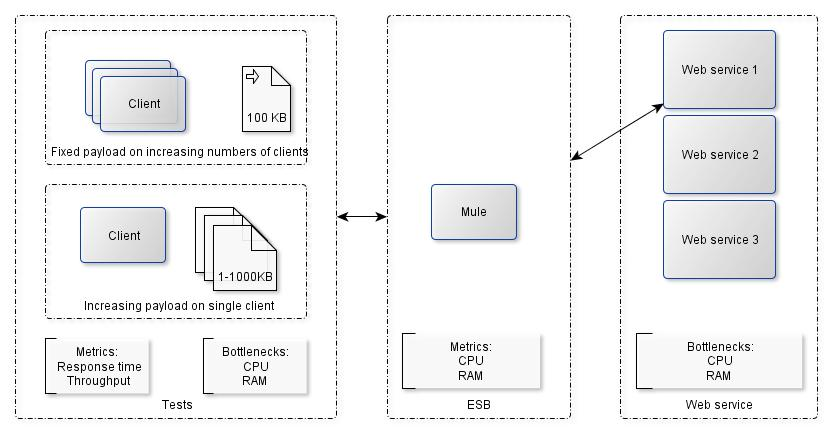
\includegraphics[scale=0.43]{img/direct_proxy}}

\subsection{Routing}
In this test the ESB will, depending on the context of an incoming request from the Client, send the request to an appropriate web service which will append some data and return the request to the ESB which will send the response to the Client.

This represents the ability to have several systems behind an ESB all showing the same front to the outside.

\centerline{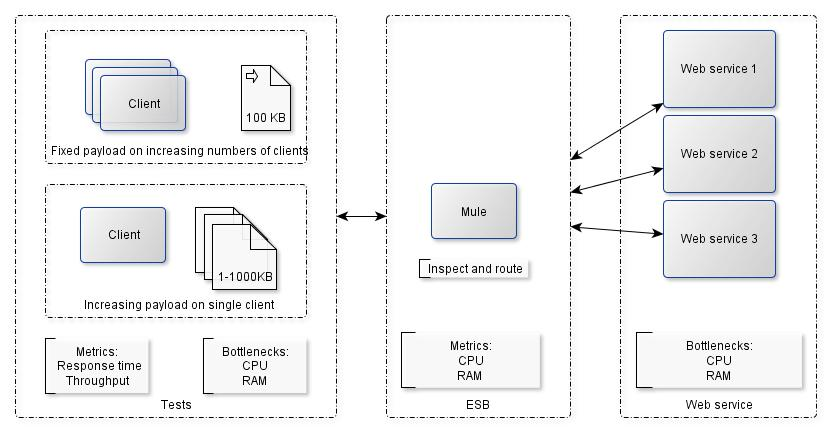
\includegraphics[scale=0.43]{img/Routing}}
\subsection{Message transformation}
The ESB will convert an incoming request to a different format and send it to a web service which will append some data and return the request to the ESB which will transform it back into the format the Client originally sent it.

\centerline{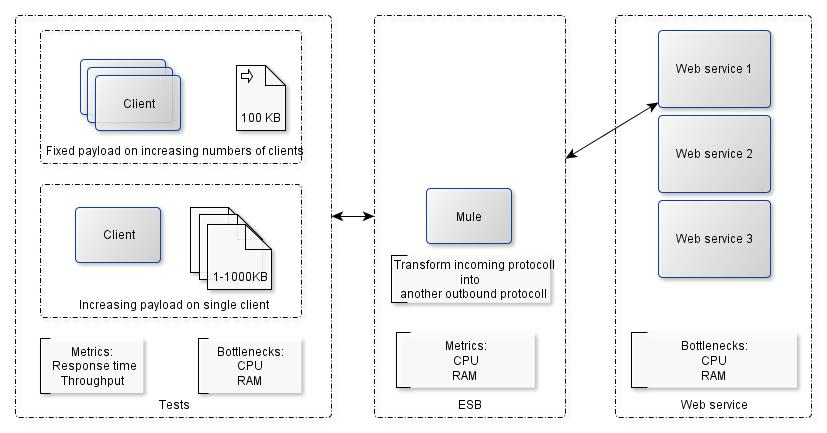
\includegraphics[scale=0.43]{img/transformation}}
\subsection{Artifacts and tools}
\begin{itemize}
	\item Client: Grinder \cite{whatisgrinder, kod}
	\item ESB: Mule \cite{whatismule, kod}
	\item Web service: Jax-WS \cite{whatisjaxws, kod}
	\item OS: Windows 7, 6.1.7600 build 7600
\end{itemize}

\subsection{Hardware setup}
In order to minimize the amount of factors that interfere in the tests we consider having at least three similar state of the art computers, connected to a high-speed network, essential.
It might not be of the greatest importance that the computers are state of the art but in order to not reach a hardware ceiling while testing, such machines are recommended. 
What's most important is that one computer is designated to run ESBs, one is designated to generate traffic(called Client) while the others are simple servers responding to the traffic generated (called Web service). 

% TODO: fixa en lista över hårdvaran (CPU,RAM,HDD osv osv)

This separating and designating of roles to machines minimizes different hardware affecting test results as the same machines perform the same roles in all tests and the only thing changed is the ESB. 

It also means that if other machines are used in other tests the data produced can be compared to ours and as such validate the data or identify faults in the tests. 
This validation can be done in two ways. 
First is to run the same software versions and compare the results. 
They should be similar deviating only in magnitude. The second is if using a newer or old software version the values when put in a graph will either have the same shape or show areas in which performance has changed, 
if it is the same shape but the magnitude is higher then that is most likely caused by faster machines being used and vice versa if its the same magnitude except in certain areas then that shows an improvement in the software.

\subsection{Variables and variable control}
No limitiations has been forseen except for hardware and notwork.
Hardware and network loads should be monitored so they are not close too 100\% as that would mean there is a major bottleneck present. 
All involved computers a run with the same operating system.
\subsection{Experiment schedule and execution sequence}
The three tests have two different focuses. First is to test scalability with an increasing amount of simulated clients (1, 20, 40, 80, 160) sending concurrent requests. 
The other is to test load-handling where a single client will send varying sizes of payload, 1KB, 50KB, 100KB, 500KB and 1MB.
\subsection{Validity threats}
This section discusses different validity threats.
\subsubsection{Different operating systems}
%Different operating system will effect test results 
%TODO säkerställ att unix inte påverkar resultaten nämnvärt
kan påvera men vi kommer att köra testerna på lite olika system så vi har ett hum om vilka förändringar det innebär i datan.
\subsubsection{Different hardware}
%TODO kör testerna en gång på /// så vi inte påverkas för mycket av hårdvara
see "different operating systems"
\subsubsection{Inefficient code}
We are not expert in the various programming languages and systems used to perform these tests and as such our code might be inefficient and even wrong. Inefficient code is not a problem as long as the same code is used in all tests. Erroneous code however is unmaintainable code and as such will require too be changed in the future and that will most likely affect the test results and test history. 
The possibilities of erroneous code has been limited by focusing the tests on very simple and basic functionality that doesn't require expert knowledge of the ESB in order to get results.
By actually providing the source code we have opened up the possibility for improvements and additions of more advanced tests which we feel is extremely important for a consistent testing framework used in academia and industry.